\begin{figure}
\centering
  \subfigure[] { 
    \label{fig:gestalt-proximity} 
    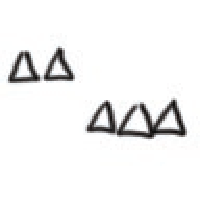
\includegraphics[width=2cm]{img/gestalt-proximity.pdf} 
  }
  \hspace{2mm}
  \subfigure[] { 
    \label{fig:gestalt-similarity} 
    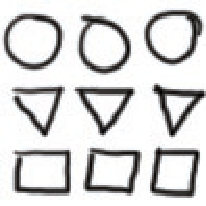
\includegraphics[width=2cm]{img/gestalt-similarity.pdf}
  }
  \hspace{2mm}
  \subfigure[] { 
    \label{fig:gestalt-symmetry} 
    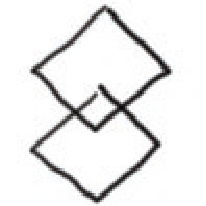
\includegraphics[width=2cm]{img/gestalt-symmetry.pdf}
  }
  \hspace{2mm}
  \subfigure[] { 
    \label{fig:gestalt-continuation} 
    
\includegraphics[width=2cm]{img/gestalt-continuation.pdf}
  }
  \hspace{2mm}
  \subfigure[] { 
    \label{fig:gestalt-closure} 
    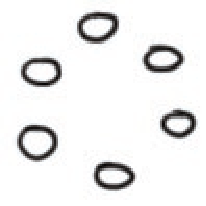
\includegraphics[width=2cm]{img/gestalt-closure.pdf}
  }

\caption[Gestalt perceptual organization]{Some principles of
  perceptual organization~\cite{kanizsa-gestalt}.
  \subref{fig:gestalt-proximity} Proximity: elements near one another
  are seen as belonging to a group. \subref{fig:gestalt-similarity}
  Similarity: objects sharing features such as shape belong in the
  same group. \subref{fig:gestalt-symmetry} Symmetry: two shapes
  symmetric about horizontal and vertical axes, suggesting they belong
  together. \subref{fig:gestalt-continuation} Continuation: the
  simplest explanation is two straight lines, not four lines meeting
  in the middle. \subref{fig:gestalt-closure} Closure: A large circle
  emerges from an arrangement of smaller circles.}
\label{fig:gestalt}
\end{figure}
